\documentclass{article}

% =====================================================================
%  WORKSHOP SWITCH -- uncomment exactly ONE of the two lines below.
%  Everything that differs between the two submissions (title, venue
%  string, abstract, intro, discussion) lives in that file; the rest of
%  this document is shared verbatim.
% =====================================================================
\newcommand{\WKFILE}{workshop-ai4good}
%\newcommand{\WKFILE}{workshop-privacy}
% =====================================================================

% ---------------------------------------------------------------------
%  ANONYMITY SWITCH.  `dblblindworkshop` prints "Anonymous Author(s)"
%  and ignores the \author block below entirely, so the real names can
%  stay in the source at all times.  For a single-blind venue or the
%  camera-ready, swap in `sglblindworkshop` and the block prints.
% ---------------------------------------------------------------------
% natbib has to be loaded with its options *before* neurips_2026 pulls it in
% bare, or the [numbers] option arrives too late. Numbered citations save
% roughly a line per paragraph of related work over author-year.
\usepackage[numbers,sort&compress]{natbib}
\usepackage[dblblindworkshop]{neurips_2026}
%\usepackage[sglblindworkshop]{neurips_2026}

\usepackage[utf8]{inputenc}
\usepackage[T1]{fontenc}
\usepackage{hyperref}
\usepackage{url}
\usepackage{booktabs}
\usepackage{amsfonts}
\usepackage{amssymb}
\usepackage{amsmath}
\usepackage{nicefrac}
\usepackage{microtype}
\usepackage[dvipsnames]{xcolor}
\usepackage{graphicx}
\usepackage{soul}

\newcommand{\martine}[1]{\textcolor{magenta}{Martine: #1}}
\newcommand{\s}[1]{\textcolor{Dandelion}{Steven: #1}}

% ---------------------------------------------------------------------
%  Numbers produced by the rf-2026-09-01 sweep. Regenerate with
%  `python manuscript/make_figs_v2.py`, which prints each of them, and
%  update here rather than in the running text.
% ---------------------------------------------------------------------
\newcommand{\CFAUCKEPT}{TKTK}      % AUC under CF / AUC under no mechanism
\newcommand{\AUCMARG}{TKTK}        % marginals-based TSTR AUC, Adult
\newcommand{\AUCDIFF}{TKTK}        % causal diffusion TSTR AUC, Adult
\newcommand{\AUCREAL}{TKTK}        % train-on-real AUC, Adult

\input{\WKFILE}

\title{\wkTitle}
\workshoptitle{\wkVenue}

\author{%
  Steven Golob\thanks{Corresponding author.} \\
  University of Washington Tacoma \\
  \texttt{golobs@uw.edu} \\
  \And
  Sikha Pentyala \\
  University of Washington Tacoma \\
  \And
  Martine De Cock \\
  University of Washington Tacoma \\
}

\begin{document}

\maketitle

\begin{abstract}
\wkAbstract
\end{abstract}

% =====================================================================
\section{Introduction}
% =====================================================================

\s{After everything else is completely finished: need to go through and remove all em dashes (replace with semi colon, parantheses, or rephrasings)}

\s{look for red text and remove the red coloring}

\wkIntro

% =====================================================================
\section{Background and related work}
\label{sec:related}
% =====================================================================

\begin{figure}[t]
  \centering
  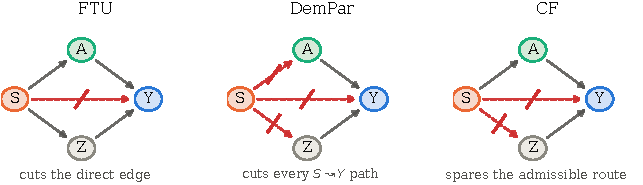
\includegraphics[width=\textwidth]{figs/pruning.pdf}
  \caption{Three fairness definitions as three sets of severed edges, acting on
  the graph the data is \emph{generated} from, not on the model trained
  afterwards for a downstream task. $S$ is the protected attribute, $Y$ the outcome, $A$ an
  admissible attribute whose influence is deemed legitimate, and $Z$ an
  intermediate proxy. Dashed red edges are cut. DemPar removes every directed
  $S \rightsquigarrow Y$ path; CF removes only those that avoid $A$, so the
  route $S \rightarrow A \rightarrow Y$ survives. \s{since we show that number of cuts goes FTU < CF < DemPar, please order the three diagrams this way, instead of "DemPar" in the middle. Also, the labels above each of the three diagrams are not centered over the diagram, and the "S" node in the diagrams are all slightly cut off on the left side, which needs to be fixed.}}
  \label{fig:pruning}
\end{figure}


\paragraph{DECAF: fairness as graph surgery.}
DECAF \citep{vanbreugel2021decaf} generates fair synthetic tables from a GAN
whose generator is \emph{factored} along a causal DAG (directed acyclic
graph): the joint distribution over columns is written as a product of
conditionals, $P(X) = \prod_i P(X_i \mid \mathrm{pa}(X_i))$, with
$\mathrm{pa}(X_i)$ the columns the graph draws as parents of column $X_i$.
This is the same decomposition a marginals-based synthesizer such as MST
\citep{mckenna2021mst} fits, differing chiefly in that MST's dependency
graph is undirected. DECAF gives each column its own sub-network reading
only $\mathrm{pa}(X_i)$, so a parent can be severed at generation time by
substituting a surrogate value drawn independently of the rest of the row.

It is worth being precise about what that costs, because DECAF describes it
as requiring no retraining. Nothing is re-estimated: the sub-network's
weights are untouched and its conditional is never re-fit. Severing
$X_j \rightarrow X_i$ instead \emph{evaluates} the trained conditional at a
parent value resampled from $X_j$'s own marginal, independently of $X_i$'s
other parents --- a \emph{do}-style intervention applied at sampling time
rather than a new model. That is exactly why the cut is cheap, and also why
it can cost fidelity: the sub-network is being asked about parent
combinations it never saw in training.

Which edges to sever turns a fairness \emph{definition} into an
\emph{algorithm}, and DECAF supplies three (Figure~\ref{fig:pruning}).
\textbf{FTU} (fairness through unawareness) cuts only the direct edge $S
\rightarrow Y$; \textbf{DemPar}\footnote{DECAF calls this mechanism DP; we
write DemPar throughout and reserve DP for differential privacy, discussed
alongside it in every result below.} (demographic parity) cuts every directed
path $S \rightsquigarrow Y$; \textbf{CF} (conditional fairness) spares paths
that pass through an attribute the modeller has nominated \emph{admissible},
so disparity routed through a legitimate factor survives. DECAF's own
illustration is the clearest: $\textit{Education} \rightarrow \textit{Resume}
\rightarrow \textit{Job}$ is worth keeping because \textit{Resume} is
admissible, while $\textit{Race} \rightarrow \textit{Postcode} \rightarrow
\textit{Loan}$ is redlining and is not. The machinery is clean, and its
authors argue it should port to other generators.

\paragraph{Differential privacy.}
Institutions releasing sensitive tables increasingly attach a differential
privacy (DP) guarantee \citep{dwork2006calibrating}: the 2020 US Census was
released under one \citep{abowd2022topdown}, and the synthesizers we study
here are the winners and entrants of the public challenges that made private
tabular release practical \citep{nist2018challenge,mckenna2021mst,vos2024}.
DP caps the influence any single individual can have on the released table by
a budget $\varepsilon$: smaller $\varepsilon$ means stronger privacy and
noisier releases. $\varepsilon{=}1$ is the tight budget an institution might
publish under; $\varepsilon{=}1000$ is a permissive comparison point that
approximates no privacy at all. Every mention of ``private'' or ``DP-''
below refers to such a synthesizer.

\paragraph{Related approaches, and the gap.}
Only one prior system attaches an in-generator fairness cut to a private
synthesizer. PreFair \citep{pujol2023prefair} adapts the CF definition above
to MST \citep{mckenna2021mst}, excluding offending marginals from candidacy
before the private structure search runs; it implements only that one
definition, and is neither built nor evaluated for any synthesizer other than
MST. Everything else that combines privacy with fairness for generation acts
outside the graph: enforcing statistical independence on a learned
intermediate embedding \citep{hyrup2025flip,sarmin2025pfwgan}, prompting an
LLM backbone \citep{nagesh2025faircausesyn}, learning a private structure
without a fairness objective \citep{jia2025pradagan}, or mitigating
downstream of the synthesizer \citep{angelozzi2026where}. Causal-DAG
diffusion generates column by column much as DECAF does, but targets fidelity
and names no protected attribute at all
\citep{zhang2025causaldifftab,jacob2026tabscm}, and private tabular diffusion
without a causal graph exposes no per-column edge to cut, so it cannot host
the mechanism at all \citep{zhu2024dptldm}.

Of these, only the downstream mitigators are measured in the units we
measure, so \citet{angelozzi2026where} is the comparison we run
(\S\ref{sec:downstream}); the embedding- and LLM-based generators report
neither a parity gap on a held-out real population nor a marginal-fidelity
score, and putting them on our axes would mean reimplementing them rather
than comparing to them. That comparison is also the one that matters, because
the downstream mitigators are the alternative a publisher actually has today
--- and, as we show, the one thing they cannot do is travel with the released
table. \s{this paragraph is worded confusingly... it's not obvious that the "embedding" thing and the LLM-backbone thing mentioned here is the same as those references in the preceding paragraph. Also, this benefit of being able to "travel with the released
table" makes no sense and has no meaning yet for a reader, and even after you explain it later, it comes across as a very specific, inconsequential benefit / shortcoming. We need to find a way to simplify this paragraph and say it more plainly and tangibly. Also, just because those other methods don't implement a certain metric isn't a strong enough reason not to not compare against them. Can we argue that angelozzi2026where is sufficient, or that hyrup2025flip, sarmin2025pfwgan, or nagesh2025faircausesyn don't have public implementations or something? Or argue why theyre not applicable, or perhaps why a comparison is not needed. it needs to be a simple, convinccing explaination. You can present a few ideas to me in the terminal claude-code session, and I will choose one.}

That leaves the question nobody has asked: is DECAF's edge surgery a property
of the complete \emph{DECAF} architecture, or of \emph{causal factorisation}? DECAF conjectures the
latter, calling the method ``simple and extendable to other generative
methods'', but never tests it. Answering this yeilds a concrete benefit: if the
mechanism is confined to DECAF, then a publisher who wants a fair release
must accept a non-private GAN that, on our own measurements
(Figure~\ref{fig:results}), no institution would deploy; if it is a property
of the factorisation, the publisher keeps the fairness lever while choosing a
synthesizer with privacy guarantees and with superior quality. And the mechanism should transfer to
the marginals-based synthesizers that dominate private tabular data \citep{mckenna2021mst, mckenna2022aim, zhang2014privbayes, zhang2021privsyn}, and to diffusion, which recent
work has shown to lead on several tabular-quality benchmarks \citep{kotelnikov2023tabddpm}.

% =====================================================================
\section{Porting the mechanisms}
\label{sec:method}
% =====================================================================

We implement FTU, DemPar and CF once, against a single
interface,\footnote{Anonymized code, with instructions to reproduce every run
and table: \url{https://anonymous.4open.science/r/CausalFairnessInSDG-55EC/}.}
and port that interface to nine generators from three unrelated families. The
fairness definitions do not change. What changes is the graph the cut acts on,
and whether that graph is directed or undirected.

\textbf{Marginals-based} synthesizers --- MST \citep{mckenna2021mst},
PrivBayes \citep{zhang2014privbayes}, PrivSyn \citep{zhang2021privsyn} and
AIM \citep{mckenna2022aim}\footnote{AIM appears only in the comparison of
\S\ref{sec:downstream}, not in the headline experiments. \s{it looks like in Table 4, and the results section, that we don't even evaluate on AIM any more. If so, remove this citation everywhere.}} --- form a graphical model
whose edges are the pairs of columns whose noisy joint counts the synthesizer
chooses to measure under the privacy budget; the release is drawn from a
distribution reproducing those counts. Their graph is undirected, so we
enforce the cut on \emph{paths} rather than on ordered
parent\,$\rightarrow$\,child edges. Whether adding a candidate pair would
create a forbidden $S$-to-$Y$ path depends on what the model already
contains, so we check the constraint incrementally at each selection step. A
pair the cut excludes is never measured, which makes the constraint free in
the privacy accounting rather than merely cheap.\footnote{The freed
$\varepsilon$ does not buy the release a better fit. MST fixes its per-round
budget from the number of edges a spanning tree needs, before selection
begins, so pruning candidates shrinks each round's pool rather than enriching
what remains; matched-pair $2$-way TVD is in fact slightly worse under the
cut, by $0.008$ for DemPar, $0.003$ for CF and $0.001$ for FTU on Adult.}

\textbf{Causal GANs} --- DECAF, plus variants we build on a CTGAN
representation \citep{xu2019ctgan} and on DP-SGD \citep{abadi2016dpsgd} ---
take DECAF's surrogate substitution unchanged, on the directed DAG. For
\textbf{causal diffusion} we keep the same factorisation and replace each
sub-network with a small denoiser trained by supervised noise prediction. The
cut is then the same code path, because what exposes an edge is that $X_i$ has
its own network reading only $\mathrm{pa}(X_i)$ --- true whether that network
was trained adversarially, as in the GAN families, or by denoising.

\paragraph{Experimental setup.}
Two datasets, Adult \citep{becker1996adult} and COMPAS
\citep{angwin2016machinebias}; nine generators; four mechanisms
(\textsc{none}/FTU/DemPar/CF); three protected/admissible role splits per
dataset (Table~\ref{tab:roles}); five seeds; $2{,}520$ completed runs. Six of
the nine generators carry a differential-privacy guarantee
\citep{dwork2006calibrating} and are marked $\dagger$ throughout: the four
marginals-based synthesizers, which are private by construction, and the three
backbones to which we attach DP-SGD (DP-GAN, DP-CTGAN, DP-Diffusion). Those
six run at $\varepsilon \in \{1,10,1000\}$ with $\delta = 10^{-9}$; DECAF,
$+$CTGAN and $+$Diffusion have no privacy mechanism and run once. For the
causal GAN and diffusion families we specify each dataset's DAG by hand from
domain knowledge, as is standard in this literature (following
\citet{kusner2017counterfactual} and \citet{zhang2017causalframework}), and
hold it fixed across generators so that any effect is attributable to the
mechanism. The marginals-based generators choose their own undirected graph
under the privacy budget, and we enforce the cut on that graph.

\begin{table}[t]
  \caption{The three role splits per dataset. \emph{Protected} is $S$,
  \emph{admissible} is $A$ (the attributes CF is allowed to route disparity
  through), and the outcome $Y$ is \texttt{income} on Adult and
  \texttt{two\_year\_recid} on COMPAS. The first split of each dataset follows
  PreFair's Table~1; the others widen and narrow the admissible set, since a
  narrow admissible set should make CF behave more like DemPar.}
  \label{tab:roles}
  \centering
  \footnotesize
  \setlength{\tabcolsep}{4pt}
  \begin{tabular}{@{}l p{0.28\textwidth} p{0.50\textwidth}@{}}
    \toprule
    Split & Protected $S$ & Admissible $A$ \\
    \midrule
    \multicolumn{3}{l}{\textit{Adult}} \\
    PreFair       & \texttt{sex}, \texttt{race}, \texttt{native-country} & \texttt{workclass}, \texttt{education}, \texttt{occupation}, \texttt{hours-per-week}, \texttt{capital-gain}, \texttt{capital-loss} \\
    Broad         & \texttt{sex} & \texttt{workclass}, \texttt{education}, \texttt{education-num}, \texttt{occupation}, \texttt{hours-per-week} \\
    Narrow        & \texttt{sex}, \texttt{race} & \texttt{education-num}, \texttt{hours-per-week} \\
    \addlinespace[2pt]
    \multicolumn{3}{l}{\textit{COMPAS}} \\
    PreFair       & \texttt{sex}, \texttt{race} & \texttt{c\_charge\_degree}, \texttt{priors\_count} \\
    Broad         & \texttt{race} & \texttt{c\_charge\_degree}, \texttt{priors\_count}, \texttt{juv\_fel\_count}, \texttt{juv\_misd\_count} \\
    Narrow        & \texttt{sex}, \texttt{race}, \texttt{age\_cat} & \texttt{c\_charge\_degree} \\
    \bottomrule
  \end{tabular}
\end{table}

\paragraph{The fairness metric.}
Every fairness number in this paper is a \textbf{demographic-parity gap}.
Train a classifier on the released synthetic table, use it to predict the
outcome for a held-out sample of \emph{real} people, and compare how often it
says yes to each protected group:
\[
  \mathrm{gap} \;=\; \bigl|\;\Pr(\hat{Y}{=}1 \mid S{=}1)\;-\;\Pr(\hat{Y}{=}1 \mid S{=}0)\;\bigr| ,
\]
reported as the worst case over the protected attributes of the split. For
example, if a classifier trained on a synthetic Adult table predicts
above-\$50k income for $50\%$ of the men and $17\%$ of the women in the real
held-out sample, the gap is $0.33$; a mechanism that brings it to $0.05$ has
removed $85\%$ of the gap. Note what the gap does and does not say: it asks
only whether the two groups receive the positive prediction equally often, not
whether either prediction is correct. It is the right target here because it
is the disparity DemPar is defined to remove, and because it is measured on
real people rather than on the synthetic table, so a generator cannot score
well by inventing a fairer population than the one it was given. We also
record conditional parity and positive- and negative-rate balance for every
run; every claim below holds on all four, and we report the parity gap because
it is the one the three mechanisms are defined against.

\paragraph{Fidelity, utility, and matched pairs.}
For \emph{fidelity} we report total-variation distance (TVD) between the
synthetic and real marginals --- half the summed absolute difference between
the two distributions, so $0$ means they agree exactly and $1$ that they share
no mass --- averaged over single columns ($1$-way) and over column pairs
($2$-way), alongside the mean absolute difference in Cram\'er's $V$ across
column pairs, which asks whether the release preserves the \emph{strength} of
each pairwise association rather than its marginal.

For \emph{utility} we train a classifier on the synthetic table and score it
on the real held-out $30\%$ \s{what is the classifier doing? You don't mention which label it is predicting? Do we do multiple labels and average the scores? This isn't written clearly.}. We report AUC and macro-F1 rather than accuracy
alone, because Adult's majority class is already $75\%$ and a real-data
classifier reaches only $82\%$: the entire learnable band is seven accuracy
points wide, which compresses good and useless generators together and pushes
several below the majority baseline for reasons that have nothing to do with
their quality \s{This is sooo tangential and needs to be cut. For a reader / reviewer, it just raises more questions about the quality and conclusions of our work!!}. AUC has a floor of $0.5$ and macro-F1 a floor of $0.41$ that a
signal-free release actually falls to, and we give both against the
train-on-real reference so a number is readable as a fraction of what the real
data supports.

Seed noise rivals the effects themselves (median within-cell SD of the parity
gap: $0.031$ on Adult, $0.092$ on COMPAS \s{this is not a good sentence. The context and scale of these numbers is not clear. What are these in reference / compared to? It is just making it harder and more arduous for the reader to get through. Can you please try to tactfully simplify your explainations to not have all of these unnecessary discrepencies?}), so every fairness number below is a
\textbf{matched-pairs} difference: each run with a fairness mechanism is
differenced against the run identical in dataset, generator, $\varepsilon$,
role split \emph{and} seed, but with no fairness mechanism.


% =====================================================================
\section{Results}
\label{sec:results}
% =====================================================================

\begin{figure}[t]
  \centering
  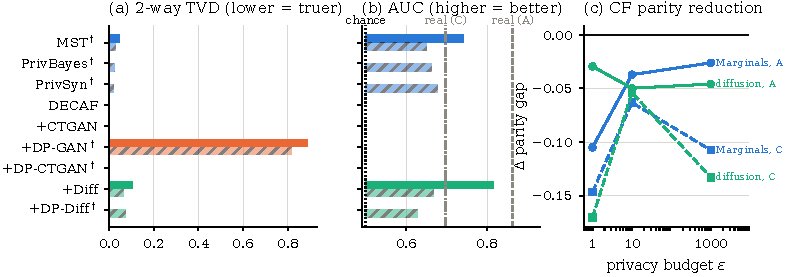
\includegraphics[width=\textwidth]{figs/results.pdf}
  \caption{\textbf{(a,\,b)} every generator with no fairness mechanism, averaged
  over $\varepsilon$, role splits and seeds; (a) $2$-way TVD to the real table
  (lower is better), (b) MLP lift over the majority-class rate (higher is
  better). A bar at zero in (b) means the data taught a classifier nothing, and
  a table with no signal has no disparity left to remove. \textbf{(c)} the
  matched-pairs reduction in parity gap from CF at each budget, for the two
  families present in every cell (marginals and diffusion; the causal GAN
  family lacks a matched cell at every budget because DP-GAN and DP-CTGAN
  collapse to a constant predictor in several cells). More negative is fairer,
  and the effect does not decay as $\varepsilon$ tightens. Each line is
  labelled with its family and dataset (A = Adult, C = COMPAS). \s{I prefer the image you had before, with the 5-element key; marginals-based, gan, diffusion, adult, compas... that was clear to me. Also, you should not just omit bars from these two bar plots, because, even though you explain it in the caption, it just looks like those have 0 value, which is misleading.} \s{can maybe mention the dagger again here and what that means, super breifly. This figure 2b that you have here is confusing. When you revert it / update it, make sure that all of the prose that references it is carefully corrected to match it.}}
  \label{fig:results}
\end{figure}

\subsection{Fidelity and utility}

Fidelity separates the nine generators cleanly (Figure~\ref{fig:results}a).
The marginals-based synthesizers dominate, as expected since they optimise
almost exactly $2$-way TVD: MST reaches $0.048$ on Adult and $0.030$ on
COMPAS. Diffusion is the next tier \s{again, doesn't this quality metric contradict the recent literature that diffusion has best tabular fidelity. Need to be more precise in such claims, that "our metric shows" or something like that, if this is unique to 2-way TVD, etc. which is just a very small window into actual, holistic fidelity.} and holds it at every privacy level: our
non-private diffusion \hl{port} \martine{What do you call it a ``port''? Is it because you use the DAG from DECAF again in the diffusion model?} reaches $0.103$ on Adult against DECAF's own
$0.544$, and with DP-SGD attached, DP-diffusion at $0.346$ still leads
DP-GAN at $0.439$ and DP-CTGAN at $0.830$.

Utility is the load-bearing panel for what follows (Figure~\ref{fig:results}b). \martine{What are the accuracies for train on real--test on real?}
Most generators clear the majority-class baseline meaningfully: on Adult
PrivBayes reaches $0.05$ lift over the $0.758$ majority-class rate \martine{So the accuracy becomes 0.808? I feel like you should say once explicitly that the accuracy when training on the synthetic data is 80\% because otherwise it may feel like $0.05$ is a tiny number.}, PrivSyn
$0.05$, our non-private diffusion port $0.04$, and DP-diffusion at
$\varepsilon\geq10$ sits just above baseline. \hl{Two cells are trouble:} \martine{Looking at Fig.~2b, DECAF, DP-CTGAN, and DP-Diff also have stuff on the left (i.e.~accuracies below the baseline); it's not so clear to me why you call out MST and DP-GAN as troublesome but not those other 3} \s{agreed. This isn't clear. The results in fig 2.b. seem a little all over the place, and maybe we need TSTR ratio, or need to redo the accuracy experiments with RF, or a different outcome / label feature? Seems very bizarre the a diffusion generator accuracy DP-diff is so far below baseline... Need to fix this, or report something else since there's no reasonable explanaition for it..} MST on
Adult sits at exactly zero lift (accuracy $0.747$, majority rate $0.758$),
and the DP-GAN family collapses to a constant predictor in several
$\varepsilon{=}1$ cells. A table that teaches a classifier nothing has no
disparity for a fairness mechanism to remove, and is scored as perfectly
fair by every existing fairness metric. Every fairness claim below is a
matched-pair difference holding the generator fixed, so this artefact does not
confound the mechanism's effect; it does mean an absolute fairness number is
uninterpretable without the utility number beside it for those two cells.

\begin{figure}[t]
  \centering
  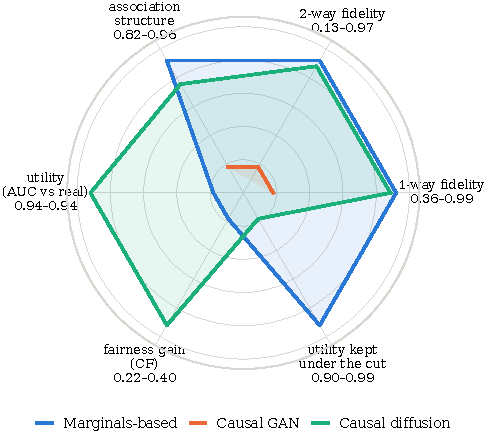
\includegraphics[width=0.52\textwidth]{figs/radar.pdf}
  \caption{The three generator families on six axes, at $\varepsilon{=}10$ for
  the differentially private generators and averaged over both datasets, all
  role splits and all seeds. Higher is better on every axis, and each axis is
  scaled between the weakest and strongest family, whose true values are
  printed beside its label --- so the shape compares families and the numbers
  give the absolute scale. \emph{Fairness gain} is the share of the baseline
  parity gap CF removes, over pairs where there was a gap to remove;
  \emph{utility kept under the cut} is downstream AUC under CF relative to the
  same generator with no mechanism, and it is the axis that says whether the
  mechanism is affordable. \s{I keep bringing up the problem of "fairness gain" making marginals-based methods look week. Can you address this? Indeed, it hides the fact that they are already more fair to begin with. So you can have a fairness gain metric here, but it needs to be accompanied by total fairness after the mechanism is applied, so that marginals-based don't look so unfair. In the prose, you could explain the low "gain" because (as table \ref{tab:edges} shows) the marginals-based application of this method removes fewer edges on average, thus changing the graph less.} \s{if you are not incorporating this graph into a panel of other graphs, then please move it to the left or right edge and make the text wrap around it... there currently is a large amount of unused white-space on either side.} \s{it looks like the utility range "0.94-0.94" is 0... that doesn't seem right...} \s{What about 2 radar plots, one for CF, one for DemPar? }}
  \label{fig:radar}
\end{figure}

\subsection{Fairness: the definitions transfer, the magnitude does not \s{maybe change the subtitle to "Fairness: the definitions transfer, with greater benefit in X family" or something like that... or even just "Fairness findings" since the two clauses to follow are used as paragraph headers below.}}

\begin{table}[t]
  \caption{Matched-pairs effect of each mechanism on the worst-case
  demographic-parity gap, pooled within generator family. \emph{gap} and
  \emph{acc} are what remains after the mechanism, both measured on real
  held-out people; the parenthesised value beside each is the mean
  \emph{paired} change against the identical run with no mechanism (negative
  = the gap shrank), with a 95\% CI on the gap. Each family header gives its
  no-mechanism gap and accuracy on Adult\,/\,COMPAS. $\dagger$ marks a
  generator carrying a differential-privacy guarantee.}
  \label{tab:fairness}
  \centering
  \footnotesize
  \setlength{\tabcolsep}{4pt}
  \begin{tabular}{l cc c cc}
    \toprule
    & \multicolumn{2}{c}{\textbf{Adult}} & & \multicolumn{2}{c}{\textbf{COMPAS}} \\
    \cmidrule(lr){2-3} \cmidrule(lr){5-6}
    Mech. & gap ($\Delta$) & acc ($\Delta$) & & gap ($\Delta$) & acc ($\Delta$) \\
    \midrule
    \multicolumn{6}{l}{\textit{Marginals-based} (MST$^\dagger$, PrivBayes$^\dagger$, PrivSyn$^\dagger$); none: gap 0.143 / 0.331, acc 0.778 / 0.636} \\
    FTU    & 0.121 ($-0.022 \pm 0.020$) & 0.779 ($+0.002$) & & 0.254 ($-0.076 \pm 0.027$) & 0.639 ($+0.003$) \\
    CF     & 0.087 ($-0.056 \pm 0.020$) & 0.773 ($-0.005$) & & 0.225 ($-0.106 \pm 0.027$) & 0.625 ($-0.011$) \\
    DemPar & 0.071 ($-0.073 \pm 0.021$) & 0.745 ($-0.032$) & & 0.230 ($-0.101 \pm 0.029$) & 0.603 ($-0.033$) \\
    \addlinespace[2pt]
    \multicolumn{6}{l}{\textit{Causal GAN} (DECAF, +CTGAN, +DP-GAN$^\dagger$, +DP-CTGAN$^\dagger$); none: gap 0.074 / 0.237, acc 0.731 / 0.567} \\
    FTU    & 0.072 ($-0.003 \pm 0.006$) & 0.731 ($-0.000$) & & 0.156 ($-0.081 \pm 0.028$) & 0.565 ($-0.002$) \\
    CF     & 0.019 ($-0.055 \pm 0.019$) & 0.730 ($-0.001$) & & 0.134 ($-0.103 \pm 0.031$) & 0.550 ($-0.017$) \\
    DemPar & 0.007 ($-0.068 \pm 0.021$) & 0.728 ($-0.003$) & & 0.094 ($-0.145 \pm 0.039$) & 0.518 ($-0.049$) \\
    \addlinespace[2pt]
    \multicolumn{6}{l}{\textit{Causal diffusion} (+Diffusion, +DP-Diffusion$^\dagger$); none: gap 0.069 / 0.294, acc 0.675 / 0.614} \\
    FTU    & 0.059 ($-0.010 \pm 0.014$) & 0.671 ($-0.004$) & & 0.193 ($-0.101 \pm 0.029$) & 0.601 ($-0.013$) \\
    CF     & 0.015 ($-0.055 \pm 0.017$) & 0.660 ($-0.015$) & & 0.160 ($-0.134 \pm 0.034$) & 0.581 ($-0.033$) \\
    DemPar & 0.003 ($-0.066 \pm 0.016$) & 0.668 ($-0.007$) & & 0.126 ($-0.167 \pm 0.034$) & 0.526 ($-0.088$) \\
    \bottomrule
  \end{tabular}
\end{table}


\textbf{The definitions transfer.} In every generator family, on both
datasets and at every privacy level, cutting edges reduces the downstream
parity gap (Table~\ref{tab:fairness}: the mean matched-pair reductions are
every one signed the same way and every one comfortably outside its own
$95\%$ interval \s{what does this "95\% interval" mean?}). This answers DECAF's own conjecture in the sense that
matters first: nothing about the three definitions requires a GAN, and
nothing about them requires a supplied directed DAG \s{"directed" is already in the acronym "DAG"}.

\textbf{The magnitude does not transfer, and the pooled averages hide that.}
The pooled numbers \s{what numbers pooled are you talking about?? Youre speaking so confusingly...} look invariant at first: on Adult, CF's mean matched-pair
reduction in parity gap is $0.056 \pm 0.020$ on marginals, $0.055 \pm 0.019$
on causal GANs and $0.055 \pm 0.017$ on causal diffusion, three means
agreeing to within $0.001$ of each other. The per-generator effects \s{what is "effect"??? stop being confusing. We are dealing with dozens of metrics in this paper and a reader cannot keep track of what you're talking about if you're not explicit!} on Adult span $0.002$ (MST)
to $0.173$ (DECAF), and each family happens to contain both a generator
that reproduces the disparity in full and one whose signal has collapsed to
the majority class (Figure~\ref{fig:results}b), so the family means average
across those extremes onto the same intermediate value \s{you are spending too much time belaboring that point about the family averages being the same, but within-family generator fairness scores being highly-varied due to some generators collapsing to solely-majority class. It's important, and interesting, but you could say this in 1 sentence.}. The comparison as a fraction of
each generator's own baseline parity gap is more informative. Restricted to
matched pairs where there is disparity to remove (baseline gap $>0.05$) and
where the generator learned something (lift $>0.02$) \s{this experiment is soo restrictive and complex. Can we simplify it? The explaination is harrowing to a reader's attention, and is not straightforward. Reduce to 2 sentences}, CF removes $89\%$ of
the baseline parity gap on the causal diffusion family, $75\%$ on the causal
GAN family and $29\%$ on the marginals-based family on Adult ($43\%$, $32\%$
and $22\%$ on COMPAS). Concretely, on DECAF
diffusion under DemPar on Adult, the fraction of men in the released table
that the downstream classifier predicts to earn above \$50k differs from the
corresponding fraction for women by $0.29$ before the mechanism is applied
and $0.03$ after. On MST the same mechanism moves it from $0.11$ to $0.09$.
Variance partitioning confirms the split: which family the generator belongs
to explains essentially none of the raw reduction ($\eta^2 = 0.00$) and
about a quarter of the fraction removed ($\eta^2 = 0.25$; $n = 432$ matched
pairs in the disparity-and-signal subset) \s{this last bit, beginning "Variance partitioning" is said confusingly... I don't knwo what n is, and I think raw reduction vs fraction removed is too complex for the reader to visualize. Just choose one and report it. Don't need to explain why one metric shows more info than another!}

\textbf{The gap has a structural cause: the same definition compiles to two
operations on very different graphs.} The causal GAN and diffusion families
receive a directed DAG \s{again, "directed" is included in "DAG", and therefor redundent, isn't it?} from a domain expert and sever its edges by surrogate
substitution at sampling time. A marginals-based synthesizer receives no DAG;
it selects an undirected structure under the privacy budget, so the definition
is enforced during that selection and can only sever an edge the structure
already carries \s{a reader might ask / point out "why not just do the same thing to marginals-based where you don't modify the graph selection process, but then at sampling time, you just change the "cut" edges nodes to be some surrogate value?" If the answer is that our method preserved privacy budget, then you could mention this in a footnote.}. The two graphs carry very different amounts of
protected-to-outcome dependence (Table~\ref{tab:edges}): the hand-designed
Adult DAG puts $\approx 9$ edges on some $S$-to-$Y$ path that DemPar must
sever, whereas the private, sparse marginals graph offers only $4$. So the GAN
and diffusion families cut more edges in absolute terms but a smaller fraction
of their already-small baseline disparity, while the marginals family cuts
fewer edges but a much larger fraction of its gap \s{I thought it was the other way around; that the gap is reduced much less in marginals-based, likely due to the fact that the number of edges cut is less, thereby modifying the graph less. You didn't explain this clearly}.

\begin{table}[t]
  \caption{Mean number of edges the mechanism must sever, per run, per
  generator family. For the causal GAN/diffusion families the count is
  deterministic: it is the number of DAG edges DECAF's surrogate
  substitution would replace given each dataset's role split. For marginals
  it is the minimum edge cut needed on the baseline (no-mechanism) learned
  undirected graph to break every forbidden $S$-to-$Y$ path (paths through
  admissibles are legal under CF, hence its intermediate size). DemPar
  $\geq$ CF $\geq$ FTU by construction.}
  \label{tab:edges}
  \centering
  \footnotesize
  \setlength{\tabcolsep}{6pt}
  \begin{tabular}{l ccc c ccc}
    \toprule
    & \multicolumn{3}{c}{\textbf{Adult}} & & \multicolumn{3}{c}{\textbf{COMPAS}} \\
    \cmidrule(lr){2-4} \cmidrule(lr){6-8}
    Family & FTU & CF & DemPar & & FTU & CF & DemPar \\
    \midrule
    Causal GAN / diffusion (fixed DAG) & 0.75 & 4.00 & 8.75 & & 1.33 & 1.67 & 3.33 \\
    Marginals-based (learned graph)   & 0.58 & 2.81 & 4.24 & & 0.96 & 2.27 & 3.72 \\
    \bottomrule
  \end{tabular}
\end{table}

\textbf{The predicted ordering falls out of the data.} Ranked by parity gap
left behind, \textsc{none} $>$ FTU $>$ CF $>$ DemPar holds in five of six
(dataset $\times$ family) cells (Table~\ref{tab:fairness}). CF landing
between the other two is a substantive check on the mechanism, not a
formality: CF spares disparity routed through the admissible attribute, so
wherever the role split gives DemPar a mediator to cut and CF one to spare,
CF must recover strictly less reduction, and it does wherever the two
separate by more than seed noise. \s{this whole result, if mentioned very briefly elsewhere, can be cut, since it is a product / finding of the DECAF paper already, and slightly obvious. But important, which is why I think it should be acknowledged somewhere as a sanity check.}

\textbf{Fairness through unawareness is weak, and on Adult barely acts.}
Pooled over Adult, FTU shifts the matched-pair parity gap by only $0.013$
on average. The pooled figure is the sum of two very different behaviours:
on MST the mechanism is a literal no-op in all $45$ Adult pairs, because
the direct protected-to-income marginal is one the private structure search
never buys under our budgets and there is nothing for the filter to
exclude; on the GAN and diffusion families FTU does cut, but the influence
promptly re-routes through proxy attributes. This is the textbook criticism
of unawareness, confirmed constructively: the cheap cut fails where the two
path-based cuts, on the same generators and seeds, work. \s{Again: this whole result can be cut, since it is a product / finding of the DECAF paper already, and slightly obvious. But the MST edges not including the to-be-cut edge is important, which could be briefly mentioned elsewhere.}

\textbf{The utility cost tracks the aggressiveness of the cut}, and is modest
for the cuts worth making: pooled over Adult, DemPar costs $1.7$ accuracy
points and CF costs $0.6$; on COMPAS, $5.0$ and $1.7$. CF stays under two
accuracy points in five of six (dataset $\times$ family) cells. \s{Maybe a small comment about how the cuts do not hinder fidelity, which is a positive trait of our method. That should be the headline finding rather than "The utility cost tracks the aggressiveness of the cut"}

\subsection{How this compares to intervening downstream}
\label{sec:downstream}

\begin{table}[t]
\centering\footnotesize
\caption{\textbf{Where to intervene, on identical data.} MST synthetic
training data, real held-out test set, XGBoost, 5 seeds, all inside the
benchmark code of \citet{angelozzi2026where}. Entries are $|$parity
gap$|$\,/\,accuracy; \textbf{bold} marks the best value in each column at
the displayed precision (lower gap, higher accuracy; ties bolded together) \s{this sentence about bold not necessary, and inferrable, and can be cut}.
The eight comparison mitigators act on the released table or on the model
trained from it; our three (\textbf{in-gen (ours)}) act inside the
generator. Majority-class accuracy is $0.758$ (Adult) and $0.533$ (COMPAS) \s{should be 2 decimal places to match the table!},
so learned fair representations buy their low gap by falling to it \s{I have no idea what this sentence means... "falling to it", "buy their low gap"???}. Accuracy
in this harness is the benchmark's own metric and is reported unchanged; note
that it understates what the release carries, since Adult's majority class
alone scores $0.758$ \s{2 decimals} and a classifier trained on the \emph{real} table reaches
only $0.82$ \s{way too much detail for a caption!}. The point of the release is not to beat a model trained on the
real data --- it cannot --- but to let others build one at all without the
real records leaving the building, and Figure~\ref{fig:results}b reports AUC
for the same reason. \s{can you greatly shorten this caption. Just the essential details and the take-aways said briefly. You're currently explaining everything here rather than, or redundent to, in the main text. Just use the main text. Also, reverse the order of DemPar and Cf here so that DemPar is last. Make sure DemPar is after CF throughout the entire paper to be consistent.} \s{all of the accuracies on adult appear to be at or far below baseline! Not a single cell above baseline accuracy.... that can't be correct!}}
\label{tab:baselines}
\begin{tabular}{llcccc}
\toprule
 & & \multicolumn{2}{c}{Adult} & \multicolumn{2}{c}{COMPAS} \\
\cmidrule(lr){3-4}\cmidrule(lr){5-6}
stage & intervention & $\varepsilon{=}1$ & $\varepsilon{=}10$ & $\varepsilon{=}1$ & $\varepsilon{=}10$ \\
\midrule
 & no mitigation        & 0.068 / 0.74 & 0.073 / 0.74 & 0.109 / \textbf{0.61} & 0.190 / 0.61 \\
\addlinespace[2pt]
pre  & Reweighing         & 0.087 / \textbf{0.75} & 0.085 / \textbf{0.75} & 0.132 / \textbf{0.61} & 0.093 / 0.61 \\
pre  & Disp.\ impact rem. & 0.078 / 0.74 & 0.105 / 0.72 & 0.119 / \textbf{0.61} & 0.205 / \textbf{0.62} \\
pre  & Learned fair repr. & 0.018 / 0.72 & 0.031 / 0.70 & 0.037 / 0.50 & 0.028 / 0.51 \\
\addlinespace[2pt]
in   & Exp.\ gradient     & 0.047 / 0.74 & 0.058 / 0.74 & 0.115 / \textbf{0.61} & 0.053 / 0.60 \\
in   & Grid search        & 0.068 / 0.74 & 0.073 / 0.74 & 0.109 / \textbf{0.61} & 0.190 / 0.61 \\
\addlinespace[2pt]
post & Reject option      & 0.045 / 0.60 & 0.046 / 0.61 & 0.045 / 0.56 & 0.046 / 0.54 \\
post & Equalised odds     & \textbf{0.009} / 0.71 & 0.015 / 0.72 & \textbf{0.024} / 0.58 & \textbf{0.023} / 0.59 \\
post & Calib.\ eq.\ odds  & 0.049 / \textbf{0.75} & 0.040 / \textbf{0.75} & 0.485 / 0.56 & 0.415 / 0.57 \\
\addlinespace[2pt]
\textbf{in-gen (ours)} & FTU    & 0.073 / 0.74 & 0.062 / 0.74 & 0.087 / 0.53 & 0.155 / 0.61 \\
\textbf{in-gen (ours)} & DemPar & 0.010 / \textbf{0.75} & \textbf{0.006} / \textbf{0.75} & 0.067 / 0.53 & 0.148 / \textbf{0.62} \\
\textbf{in-gen (ours)} & CF     & 0.015 / \textbf{0.75} & 0.029 / 0.74 & 0.111 / 0.59 & 0.155 / 0.61 \\
\bottomrule
\end{tabular}
\end{table}


Everything so far measures the mechanism against itself. To place it against
the alternatives an institution actually has, we ran the benchmark of
\citet{angelozzi2026where} (introduced in \S\ref{sec:related}), which asks
where in a differentially private \s{why is differential privacy relevant to this whole section? I thought these methods were just about fairness? Why does DP enter the discussion. You need to reduce the complexity , unneccessary detail!} synthetic pipeline a fairness intervention
should go and offers eight standard answers spread across pre-processing the
table, constraining the downstream classifier, and post-processing its predictions \s{are all 8 interventions done after the synthetic data is generated? This wasn't clear to me. If so, that's more interesting. Clarify.}. We
add ours as a fourth stage, applied inside the generator. We use their code
unmodified (their preprocessed data, splits, MST synthesizer, XGBoost
classifier and aif360 metrics); the only change is that our arm's training
table comes from our MST under FTU, DemPar or CF rather than theirs \s{this sentence is bad; we don't make a "change", we just compare our method to theirs (produced from their code). The way it currently is written makes it sound like we moddled together our method with theirs, which sounds like something we haven't discussed yet in the methods section.... too confusing.}.
Table~\ref{tab:baselines} is the result.

On Adult the in-generator cut is on the fairness/accuracy frontier
(Table~\ref{tab:baselines}, columns 1--2). DemPar in-generator leaves a
parity gap of $0.010$ at $0.748$ \s{2 decimals to be consistent with the table, please! Also, isn't this accuracy below baseline!!?} accuracy; the only downstream mitigator that
reaches a comparable fairness gap is equalized-odds post-processing (which threshold-shifts the classifier per group) at $0.009$, and it costs $3.4$ more accuracy
points to get there. Reweighing and the disparate-impact remover leave the
release \emph{less} fair than no mitigation at all in this cell, and grid
search is an exact no-op. On COMPAS the ordering reverses: post-processing
reaches $0.023$ where our best cut reaches $0.148$ \s{it's not clear to me which role from table \ref{tab:roles} these are based on...}. This is the same finding
as \S\ref{sec:results} \s{we're IN section \S\ref{sec:results}! What part are you talking about?} seen from outside, since at these budgets the
privately selected MST structure barely encodes the protected-to-outcome
dependence and there is correspondingly little for a cut to sever, whereas a
mitigator acting on the trained downstream classifier is not subject to that limit \s{but what does this have to do with the difference between the COMPAS settings and the Adult settings? Why is the result inversed across the 2 datasets... that's not clear in your explaination. You are discussing something else, possibly tangential}. FTU and
CF are exact no-ops on Adult in this harness too, reproducing the FTU result
above in a different codebase and metric \s{don't know what this sentence means or why it's necessary}.

This is not a like-for-like ranking of techniques: a downstream mitigator is
applied by whoever trains a downstream model , whereas the in-generator cut is applied once
by the synthetic data publisher and is the only one of the four that ships with the released
table (discussed in Sec.~\ref{sec:discussion}).

\subsection{Privacy and fairness are nearly independent}

There is a reason to expect privacy and fairness to pull against each other.
Differential privacy suppresses the influence of any one record, so a
classifier trained under it loses the most accuracy on the groups that appear
least often \citep{bagdasaryan2019disparate}. It is natural to suspect that
the same suppression would also cost the smallest groups their fair treatment,
and that tightening $\varepsilon$ would therefore blunt any attempt to close a
parity gap. We find it does not, and the reason the suspicion does not carry
over is worth stating: the parity gap asks whether two groups receive a
positive prediction equally often, not whether either prediction is accurate,
and it is measured here on real held-out people rather than on the noisy
release. Losing accuracy on a small group and treating that group unequally
are different failures, and differential privacy causes only the first \s{so... does this mean groups are treated more fairly or equally fairly under DP?Be concrete.}. \s{We could possibly refer to the top row "no mitigation" in table \ref{tab:baselines} to show that at epsilon=1 , the fairness is already improved in MST, vs. at epsilon=10, without any fairness technique applied.}

Empirically, cutting edges reduces the parity gap at least as much at the
strong $\varepsilon{=}1$ as at the permissive $\varepsilon{=}1000$ in nine of
twelve (family $\times$ dataset $\times$ \{CF, DemPar\}) cells; \s{everything from here onward in this paragraph and in the next paragrpah, is too detailed and full of discrepancies and too many measurements. Can you simplify it to one or two clear trends only? Some data backing is good. But what you have currently is too much for a reader to hold in their head, too many variables, etc. We need to follow the larger cross-variable trends. Can you find more direct results and rewrite these two paragraphs accordingly?} two of the
three exceptions are COMPAS GAN cells where the backbone has already collapsed
to a constant predictor at $\varepsilon{=}1$ and has no disparity left to
remove. For marginals-based generators on Adult, CF's mean paired reduction in
parity gap is $0.105$ at $\varepsilon{=}1$ against $0.026$ at
$\varepsilon{=}1000$ (on COMPAS, $0.147$ against $0.108$), and it moves the
same way as a fraction of baseline ($68\%$ against $18\%$ on Adult). For
causal diffusion it is essentially flat ($0.030$, $0.050$, $0.046$ across the
three budgets on Adult).

Part of that is simply that a tight budget leaves more to remove, though less
than one might assume: the baseline parity gap on Adult marginals is $0.155$
at $\varepsilon{=}1$ against $0.147$ at $\varepsilon{=}1000$, a widening of
$0.008$, and on COMPAS $0.351$ against $0.333$. The effect is small, and it is
not universal --- COMPAS diffusion runs the other way ($0.272$ at
$\varepsilon{=}1$ against $0.336$). The same accounting explains the one
non-monotonicity \s{again, I'll point out again that, you are describing and coming up with explainations for every discrepancy in the results. but instead, throughout, we need to first find the views of the data that tell a clear story, so we don't have to spend paragraphs upon paragraphs explaining them. If you find that it takes a paragraph to explain a secondary table result, then you need to find a new angle / new aggregation / new finding from that table, or a new table alogether that shows something intuitive, and easy to interpret without raising a bunch of other questions. This is very important. Please take time to address this. Do not rush it. I want your revision to shorten the paper, with equal or greater impact.} in Figure~\ref{fig:results}c, where on \emph{both} COMPAS
lines the reduction at $\varepsilon{=}10$ is smaller than at either
neighbouring budget: the baseline gap is smallest at that budget too ($0.309$
for marginals, $0.244$ for diffusion), so there is less disparity present for
the cut to take away. Neither Adult line shows the pattern.


\textbf{One private generator fails outright}, on a claim DECAF makes. DECAF
argues from the post-processing theorem that it ``can be directly used for
generating private synthetic data by replacing the standard discriminator by
a differentially private discriminator.'' The accounting is correct; the
output is not. Attaching DP-SGD \citep{abadi2016dpsgd} to DECAF's WGAN-GP
critic in this way (the DP-GAN row in Table~\ref{tab:fairness}) collapses
the synthetic outcome to a single class in $168$ of $360$ runs ($47\%$),
every COMPAS run at $\varepsilon{=}1$ included. Two independent changes each
remove the failure: substituting a CTGAN representation under the same
adversarial training ($1/360$), and substituting diffusion for the WGAN-GP
critic \s{what is "critic"? discriminator? GAN?} under DECAF's own representation ($0/360$). Two unrelated repairs
locate the cause in DP-SGD on a weight-clipped critic \s{critic?}, not in private causal
generation as such.

% =====================================================================
\section{Discussion}
\label{sec:discussion}
% =====================================================================
\wkDiscussion

\bibliographystyle{plainnat}
\bibliography{refs}

\section*{NeurIPS Paper Checklist}

\begin{enumerate}

\item {\bf Claims}
    \item[] Question: Do the main claims made in the abstract and introduction accurately reflect the paper's contributions and scope?
    \item[] Answer: \answerYes{}
    \item[] Justification: The abstract and introduction claim that DECAF's edge-surgery fairness mechanism ports beyond its original GAN to marginals-based and diffusion generators; Sections~\ref{sec:method}--\ref{sec:results} establish exactly this across nine generators, two datasets and three privacy budgets, and we are explicit that the \emph{magnitude} of the effect does not transfer even though the definitions do.
    \item[] Guidelines:
    \begin{itemize}
        \item The answer \answerNA{} means that the abstract and introduction do not include the claims made in the paper.
        \item The abstract and/or introduction should clearly state the claims made, including the contributions made in the paper and important assumptions and limitations. A \answerNo{} or \answerNA{} answer to this question will not be perceived well by the reviewers.
        \item The claims made should match theoretical and experimental results, and reflect how much the results can be expected to generalize to other settings.
        \item It is fine to include aspirational goals as motivation as long as it is clear that these goals are not attained by the paper.
    \end{itemize}

\item {\bf Limitations}
    \item[] Question: Does the paper discuss the limitations of the work performed by the authors?
    \item[] Answer: \answerYes{}
    \item[] Justification: Limitations are discussed inline rather than in a separate section: the effect magnitude does not transfer across families and depends on the supplied or privately learned graph (\S\ref{sec:results}); two generators produce degenerate-utility tables that trivially appear fair (\S\ref{sec:results}); the reduction at $\varepsilon{=}10$ is weaker than at either neighbouring budget and we cannot yet explain it (\S\ref{sec:results}); and the causal-GAN/diffusion results rely on a hand-specified DAG (\S\ref{sec:method}).
    \item[] Guidelines:
    \begin{itemize}
        \item The answer \answerNA{} means that the paper has no limitation while the answer \answerNo{} means that the paper has limitations, but those are not discussed in the paper.
        \item The authors are encouraged to create a separate ``Limitations'' section in their paper.
        \item The paper should point out any strong assumptions and how robust the results are to violations of these assumptions (e.g., independence assumptions, noiseless settings, model well-specification, asymptotic approximations only holding locally). The authors should reflect on how these assumptions might be violated in practice and what the implications would be.
        \item The authors should reflect on the scope of the claims made, e.g., if the approach was only tested on a few datasets or with a few runs. In general, empirical results often depend on implicit assumptions, which should be articulated.
        \item The authors should reflect on the factors that influence the performance of the approach. For example, a facial recognition algorithm may perform poorly when image resolution is low or images are taken in low lighting. Or a speech-to-text system might not be used reliably to provide closed captions for online lectures because it fails to handle technical jargon.
        \item The authors should discuss the computational efficiency of the proposed algorithms and how they scale with dataset size.
        \item If applicable, the authors should discuss possible limitations of their approach to address problems of privacy and fairness.
        \item While the authors might fear that complete honesty about limitations might be used by reviewers as grounds for rejection, a worse outcome might be that reviewers discover limitations that aren't acknowledged in the paper. The authors should use their best judgment and recognize that individual actions in favor of transparency play an important role in developing norms that preserve the integrity of the community. Reviewers will be specifically instructed to not penalize honesty concerning limitations.
    \end{itemize}

\item {\bf Theory assumptions and proofs}
    \item[] Question: For each theoretical result, does the paper provide the full set of assumptions and a complete (and correct) proof?
    \item[] Answer: \answerNA{}
    \item[] Justification: The paper makes no formal theoretical claims and states no theorems; all results are empirical.
    \item[] Guidelines:
    \begin{itemize}
        \item The answer \answerNA{} means that the paper does not include theoretical results.
        \item All the theorems, formulas, and proofs in the paper should be numbered and cross-referenced.
        \item All assumptions should be clearly stated or referenced in the statement of any theorems.
        \item The proofs can either appear in the main paper or the supplemental material, but if they appear in the supplemental material, the authors are encouraged to provide a short proof sketch to provide intuition.
        \item Inversely, any informal proof provided in the core of the paper should be complemented by formal proofs provided in appendix or supplemental material.
        \item Theorems and Lemmas that the proof relies upon should be properly referenced.
    \end{itemize}

    \item {\bf Experimental result reproducibility}
    \item[] Question: Does the paper fully disclose all the information needed to reproduce the main experimental results of the paper to the extent that it affects the main claims and/or conclusions of the paper (regardless of whether the code and data are provided or not)?
    \item[] Answer: \answerYes{}
    \item[] Justification: Section~\ref{sec:method} specifies the datasets, generators, fairness mechanisms, privacy budgets, role splits, seed count, downstream classifier and matched-pairs protocol, and we release an anonymized code repository with instructions to reproduce every run and every table (footnote in \S\ref{sec:method}).
    \item[] Guidelines:
    \begin{itemize}
        \item The answer \answerNA{} means that the paper does not include experiments.
        \item If the paper includes experiments, a \answerNo{} answer to this question will not be perceived well by the reviewers: Making the paper reproducible is important, regardless of whether the code and data are provided or not.
        \item If the contribution is a dataset and\slash or model, the authors should describe the steps taken to make their results reproducible or verifiable.
        \item Depending on the contribution, reproducibility can be accomplished in various ways. For example, if the contribution is a novel architecture, describing the architecture fully might suffice, or if the contribution is a specific model and empirical evaluation, it may be necessary to either make it possible for others to replicate the model with the same dataset, or provide access to the model. In general. releasing code and data is often one good way to accomplish this, but reproducibility can also be provided via detailed instructions for how to replicate the results, access to a hosted model (e.g., in the case of a large language model), releasing of a model checkpoint, or other means that are appropriate to the research performed.
        \item While NeurIPS does not require releasing code, the conference does require all submissions to provide some reasonable avenue for reproducibility, which may depend on the nature of the contribution. For example
        \begin{enumerate}
            \item If the contribution is primarily a new algorithm, the paper should make it clear how to reproduce that algorithm.
            \item If the contribution is primarily a new model architecture, the paper should describe the architecture clearly and fully.
            \item If the contribution is a new model (e.g., a large language model), then there should either be a way to access this model for reproducing the results or a way to reproduce the model (e.g., with an open-source dataset or instructions for how to construct the dataset).
            \item We recognize that reproducibility may be tricky in some cases, in which case authors are welcome to describe the particular way they provide for reproducibility. In the case of closed-source models, it may be that access to the model is limited in some way (e.g., to registered users), but it should be possible for other researchers to have some path to reproducing or verifying the results.
        \end{enumerate}
    \end{itemize}


\item {\bf Open access to data and code}
    \item[] Question: Does the paper provide open access to the data and code, with sufficient instructions to faithfully reproduce the main experimental results, as described in supplemental material?
    \item[] Answer: \answerYes{}
    \item[] Justification: Both datasets (Adult, COMPAS) are public, and we release an anonymized code repository with the synthesizer/mechanism implementations and the run and analysis scripts at \url{https://anonymous.4open.science/r/CausalFairnessInSDG-55EC/} (also cited in \S\ref{sec:method}).
    \item[] Guidelines:
    \begin{itemize}
        \item The answer \answerNA{} means that paper does not include experiments requiring code.
        \item Please see the NeurIPS code and data submission guidelines (\url{https://neurips.cc/public/guides/CodeSubmissionPolicy}) for more details.
        \item While we encourage the release of code and data, we understand that this might not be possible, so \answerNo{} is an acceptable answer. Papers cannot be rejected simply for not including code, unless this is central to the contribution (e.g., for a new open-source benchmark).
        \item The instructions should contain the exact command and environment needed to run to reproduce the results. See the NeurIPS code and data submission guidelines (\url{https://neurips.cc/public/guides/CodeSubmissionPolicy}) for more details.
        \item The authors should provide instructions on data access and preparation, including how to access the raw data, preprocessed data, intermediate data, and generated data, etc.
        \item The authors should provide scripts to reproduce all experimental results for the new proposed method and baselines. If only a subset of experiments are reproducible, they should state which ones are omitted from the script and why.
        \item At submission time, to preserve anonymity, the authors should release anonymized versions (if applicable).
        \item Providing as much information as possible in supplemental material (appended to the paper) is recommended, but including URLs to data and code is permitted.
    \end{itemize}


\item {\bf Experimental setting/details}
    \item[] Question: Does the paper specify all the training and test details (e.g., data splits, hyperparameters, how they were chosen, type of optimizer) necessary to understand the results?
    \item[] Answer: \answerYes{}
    \item[] Justification: Section~\ref{sec:method} gives the datasets, the $30\%$ real held-out test split, the downstream MLP, the three protected/admissible role splits, the privacy budgets ($\varepsilon \in \{1,10,1000\}$, $\delta = 10^{-9}$) and five seeds per cell; the remaining hyperparameters are fixed in the released code.
    \item[] Guidelines:
    \begin{itemize}
        \item The answer \answerNA{} means that the paper does not include experiments.
        \item The experimental setting should be presented in the core of the paper to a level of detail that is necessary to appreciate the results and make sense of them.
        \item The full details can be provided either with the code, in appendix, or as supplemental material.
    \end{itemize}

\item {\bf Experiment statistical significance}
    \item[] Question: Does the paper report error bars suitably and correctly defined or other appropriate information about the statistical significance of the experiments?
    \item[] Answer: \answerYes{}
    \item[] Justification: Every fairness number is a matched-pairs difference (each mechanism run is differenced against the no-mechanism run identical in dataset, generator, budget, role split and seed); Table~\ref{tab:fairness} reports mean paired changes with $95\%$ confidence intervals, and \S\ref{sec:method} reports the within-cell seed standard deviation that motivates the paired design.
    \item[] Guidelines:
    \begin{itemize}
        \item The answer \answerNA{} means that the paper does not include experiments.
        \item The authors should answer \answerYes{} if the results are accompanied by error bars, confidence intervals, or statistical significance tests, at least for the experiments that support the main claims of the paper.
        \item The factors of variability that the error bars are capturing should be clearly stated (for example, train/test split, initialization, random drawing of some parameter, or overall run with given experimental conditions).
        \item The method for calculating the error bars should be explained (closed form formula, call to a library function, bootstrap, etc.)
        \item The assumptions made should be given (e.g., Normally distributed errors).
        \item It should be clear whether the error bar is the standard deviation or the standard error of the mean.
        \item It is OK to report 1-sigma error bars, but one should state it. The authors should preferably report a 2-sigma error bar than state that they have a 96\% CI, if the hypothesis of Normality of errors is not verified.
        \item For asymmetric distributions, the authors should be careful not to show in tables or figures symmetric error bars that would yield results that are out of range (e.g., negative error rates).
        \item If error bars are reported in tables or plots, the authors should explain in the text how they were calculated and reference the corresponding figures or tables in the text.
    \end{itemize}

\item {\bf Experiments compute resources}
    \item[] Question: For each experiment, does the paper provide sufficient information on the computer resources (type of compute workers, memory, time of execution) needed to reproduce the experiments?
    \item[] Answer: \answerYes{}
    \item[] Justification: All experiments run on a single shared Linux workstation; the models are small (tabular MLPs and per-column generators/denoisers), a single GPU is used for the GAN and diffusion backbones, and the full 2{,}520-run sweep completes in roughly 6--12 hours of wall-clock time when parallelised.
    \item[] Guidelines:
    \begin{itemize}
        \item The answer \answerNA{} means that the paper does not include experiments.
        \item The paper should indicate the type of compute workers CPU or GPU, internal cluster, or cloud provider, including relevant memory and storage.
        \item The paper should provide the amount of compute required for each of the individual experimental runs as well as estimate the total compute.
        \item The paper should disclose whether the full research project required more compute than the experiments reported in the paper (e.g., preliminary or failed experiments that didn't make it into the paper).
    \end{itemize}

\item {\bf Code of ethics}
    \item[] Question: Does the research conducted in the paper conform, in every respect, with the NeurIPS Code of Ethics \url{https://neurips.cc/public/EthicsGuidelines}?
    \item[] Answer: \answerYes{}
    \item[] Justification: The research uses only public, widely studied benchmark datasets, involves no human-subjects data collection, and its goal (reducing demographic disparity in released synthetic data under privacy guarantees) is consistent with the NeurIPS Code of Ethics.
    \item[] Guidelines:
    \begin{itemize}
        \item The answer \answerNA{} means that the authors have not reviewed the NeurIPS Code of Ethics.
        \item If the authors answer \answerNo, they should explain the special circumstances that require a deviation from the Code of Ethics.
        \item The authors should make sure to preserve anonymity (e.g., if there is a special consideration due to laws or regulations in their jurisdiction).
    \end{itemize}


\item {\bf Broader impacts}
    \item[] Question: Does the paper discuss both potential positive societal impacts and negative societal impacts of the work performed?
    \item[] Answer: \answerYes{}
    \item[] Justification: The intended impact is positive: enabling institutions to remove unfair pathways from synthetic releases (Introduction, Discussion). We also flag concrete failure modes: a generator that teaches a classifier nothing has no disparity to remove yet scores as perfectly fair, so a fairness number is uninterpretable without its utility number (\S\ref{sec:results}), and an in-generator cut can give false assurance if downstream consumers assume more disparity was removed than the graph actually permitted (\S\ref{sec:results}, Discussion).
    \item[] Guidelines:
    \begin{itemize}
        \item The answer \answerNA{} means that there is no societal impact of the work performed.
        \item If the authors answer \answerNA{} or \answerNo, they should explain why their work has no societal impact or why the paper does not address societal impact.
        \item Examples of negative societal impacts include potential malicious or unintended uses (e.g., disinformation, generating fake profiles, surveillance), fairness considerations (e.g., deployment of technologies that could make decisions that unfairly impact specific groups), privacy considerations, and security considerations.
        \item The conference expects that many papers will be foundational research and not tied to particular applications, let alone deployments. However, if there is a direct path to any negative applications, the authors should point it out. For example, it is legitimate to point out that an improvement in the quality of generative models could be used to generate Deepfakes for disinformation. On the other hand, it is not needed to point out that a generic algorithm for optimizing neural networks could enable people to train models that generate Deepfakes faster.
        \item The authors should consider possible harms that could arise when the technology is being used as intended and functioning correctly, harms that could arise when the technology is being used as intended but gives incorrect results, and harms following from (intentional or unintentional) misuse of the technology.
        \item If there are negative societal impacts, the authors could also discuss possible mitigation strategies (e.g., gated release of models, providing defenses in addition to attacks, mechanisms for monitoring misuse, mechanisms to monitor how a system learns from feedback over time, improving the efficiency and accessibility of ML).
    \end{itemize}

\item {\bf Safeguards}
    \item[] Question: Does the paper describe safeguards that have been put in place for responsible release of data or models that have a high risk for misuse (e.g., pre-trained language models, image generators, or scraped datasets)?
    \item[] Answer: \answerNA{}
    \item[] Justification: The paper releases fairness-mechanism code operating on public tabular benchmarks; it releases no pre-trained generative model, scraped dataset, or other artifact with a high risk for misuse.
    \item[] Guidelines:
    \begin{itemize}
        \item The answer \answerNA{} means that the paper poses no such risks.
        \item Released models that have a high risk for misuse or dual-use should be released with necessary safeguards to allow for controlled use of the model, for example by requiring that users adhere to usage guidelines or restrictions to access the model or implementing safety filters.
        \item Datasets that have been scraped from the Internet could pose safety risks. The authors should describe how they avoided releasing unsafe images.
        \item We recognize that providing effective safeguards is challenging, and many papers do not require this, but we encourage authors to take this into account and make a best faith effort.
    \end{itemize}

\item {\bf Licenses for existing assets}
    \item[] Question: Are the creators or original owners of assets (e.g., code, data, models), used in the paper, properly credited and are the license and terms of use explicitly mentioned and properly respected?
    \item[] Answer: \answerYes{}
    \item[] Justification: Every existing asset is cited to its original source: the Adult and COMPAS datasets, the DECAF, MST, PrivBayes, PrivSyn and AIM synthesizers, DP-SGD, and the downstream benchmark of \citet{angelozzi2026where} whose code we reuse unmodified. Each is publicly released for research use, and our re-implementations credit the upstream packages they adapt.
    \item[] Guidelines:
    \begin{itemize}
        \item The answer \answerNA{} means that the paper does not use existing assets.
        \item The authors should cite the original paper that produced the code package or dataset.
        \item The authors should state which version of the asset is used and, if possible, include a URL.
        \item The name of the license (e.g., CC-BY 4.0) should be included for each asset.
        \item For scraped data from a particular source (e.g., website), the copyright and terms of service of that source should be provided.
        \item If assets are released, the license, copyright information, and terms of use in the package should be provided. For popular datasets, \url{paperswithcode.com/datasets} has curated licenses for some datasets. Their licensing guide can help determine the license of a dataset.
        \item For existing datasets that are re-packaged, both the original license and the license of the derived asset (if it has changed) should be provided.
        \item If this information is not available online, the authors are encouraged to reach out to the asset's creators.
    \end{itemize}

\item {\bf New assets}
    \item[] Question: Are new assets introduced in the paper well documented and is the documentation provided alongside the assets?
    \item[] Answer: \answerYes{}
    \item[] Justification: The one new asset is the fairness-porting codebase; it is released in the anonymized repository above with a README documenting the environment setup, the synthesizer and fairness-mechanism interfaces, and how to run the experiments.
    \item[] Guidelines:
    \begin{itemize}
        \item The answer \answerNA{} means that the paper does not release new assets.
        \item Researchers should communicate the details of the dataset\slash code\slash model as part of their submissions via structured templates. This includes details about training, license, limitations, etc.
        \item The paper should discuss whether and how consent was obtained from people whose asset is used.
        \item At submission time, remember to anonymize your assets (if applicable). You can either create an anonymized URL or include an anonymized zip file.
    \end{itemize}

\item {\bf Crowdsourcing and research with human subjects}
    \item[] Question: For crowdsourcing experiments and research with human subjects, does the paper include the full text of instructions given to participants and screenshots, if applicable, as well as details about compensation (if any)?
    \item[] Answer: \answerNA{}
    \item[] Justification: The paper uses pre-existing public datasets and involves no crowdsourcing or new human-subjects data collection.
    \item[] Guidelines:
    \begin{itemize}
        \item The answer \answerNA{} means that the paper does not involve crowdsourcing nor research with human subjects.
        \item Including this information in the supplemental material is fine, but if the main contribution of the paper involves human subjects, then as much detail as possible should be included in the main paper.
        \item According to the NeurIPS Code of Ethics, workers involved in data collection, curation, or other labor should be paid at least the minimum wage in the country of the data collector.
    \end{itemize}

\item {\bf Institutional review board (IRB) approvals or equivalent for research with human subjects}
    \item[] Question: Does the paper describe potential risks incurred by study participants, whether such risks were disclosed to the subjects, and whether Institutional Review Board (IRB) approvals (or an equivalent approval/review based on the requirements of your country or institution) were obtained?
    \item[] Answer: \answerNA{}
    \item[] Justification: No human-subjects research was conducted; the work reuses public benchmark datasets only.
    \item[] Guidelines:
    \begin{itemize}
        \item The answer \answerNA{} means that the paper does not involve crowdsourcing nor research with human subjects.
        \item Depending on the country in which research is conducted, IRB approval (or equivalent) may be required for any human subjects research. If you obtained IRB approval, you should clearly state this in the paper.
        \item We recognize that the procedures for this may vary significantly between institutions and locations, and we expect authors to adhere to the NeurIPS Code of Ethics and the guidelines for their institution.
        \item For initial submissions, do not include any information that would break anonymity (if applicable), such as the institution conducting the review.
    \end{itemize}

\item {\bf Declaration of LLM usage}
    \item[] Question: Does the paper describe the usage of LLMs if it is an important, original, or non-standard component of the core methods in this research? Note that if the LLM is used only for writing, editing, or formatting purposes and does \emph{not} impact the core methodology, scientific rigor, or originality of the research, declaration is not required.
    %this research?
    \item[] Answer: \answerNA{}
    \item[] Justification: LLMs are not a component of the core methods; the generators studied are marginals-based, GAN and diffusion models. Any LLM use was limited to writing and editing assistance, for which declaration is not required.
    \item[] Guidelines:
    \begin{itemize}
        \item The answer \answerNA{} means that the core method development in this research does not involve LLMs as any important, original, or non-standard components.
        \item Please refer to our LLM policy in the NeurIPS handbook for what should or should not be described.
    \end{itemize}

\end{enumerate}


\end{document}
